% id: 1347
% book: 라이트쎈 공통수학1 · 11 행렬과 그 연산
% section: 유형 03 행렬의 덧셈, 뺄셈, 실수배
% figure: tikz:fig-1347
% answer: ⑤
% answer_source: 답지
% variant_level: 0 (원본 전사)
% 이 파일은 build.mjs 가 items.json 에서 만든다. 고칠 때는 items.json 을 고친다.
\hspace*{2mm}\begin{minipage}[t]{\dimexpr\linewidth-2mm\relax}\vspace{0pt}\smash{\raisebox{5.5mm}{\dmkichul{라이트쎈 공통수학1 1347번 · 189쪽}}}
\noindent\begin{minipage}[t]{0.58\linewidth}\vspace{0pt}\raggedright 오른쪽 그림과 같이 행렬 $X=\begin{pmatrix} a & b \\ c & d \end{pmatrix}$의 각 행의 성분을 좌표로 하는 두 점 $(a,\,b)$, $(c,\,d)$와 원점 $\mathrm{O}$를 꼭짓점으로 하는 삼각형의 넓이를 $S(X)$라 하자. 이때 두 행렬 $A=\begin{pmatrix} 1 & 3 \\ 3 & 2 \end{pmatrix}$, $B=\begin{pmatrix} 3 & -1 \\ -1 & 0 \end{pmatrix}$에 대하여 $S(3A-B)$의 값은?\end{minipage}\hfill\begin{minipage}[t]{0.4\linewidth}\vspace{0pt}\centering \resizebox{\ifdim\width>\linewidth\linewidth\else\width\fi}{!}{% 1347(본책 189쪽) — 좌표평면에서 원점 O 와 두 점 (a, b), (c, d) 를 꼭짓점으로 하는 삼각형(넓이 S(X)) 그림. 스캔 그림이라 TikZ 로 다시 그림. 라벨은 원문 O·(a, b)·(c, d)·S(X)·x·y 만.
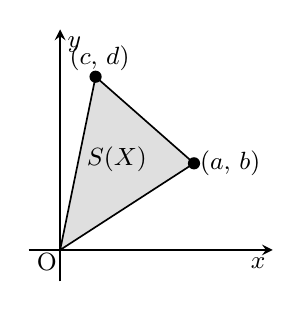
\begin{tikzpicture}[x=1cm, y=1cm, line width=0.5pt]
  \fill[gray!25] (0,0) -- (1.7,1.1) -- (0.45,2.2) -- cycle;
  \draw[->, >=stealth, line width=0.7pt] (-0.4,0) -- (2.7,0) node[below left=-1pt, font=\small] {$x$};
  \draw[->, >=stealth, line width=0.7pt] (0,-0.4) -- (0,2.8) node[below right=-1pt, font=\small] {$y$};
  \node[below left, font=\small, inner sep=1pt] at (0,0) {$\mathrm{O}$};
  \draw[line width=0.6pt] (0,0) -- (1.7,1.1) -- (0.45,2.2) -- cycle;
  \fill (1.7,1.1) circle (2.2pt);
  \fill (0.45,2.2) circle (2.2pt);
  \node[right, font=\small, inner sep=2pt] at (1.7,1.1) {$(a,\,b)$};
  \node[above, font=\small, inner sep=2pt] at (0.5,2.2) {$(c,\,d)$};
  \node[font=\small, inner sep=1pt] at (0.72,1.15) {$S(X)$};
\end{tikzpicture}
}\end{minipage}\par
\begin{choices32}{$42$}{$44$}{$46$}{$48$}{$50$}\end{choices32}\end{minipage}
